% Upload HW2-overleaf.zip to Overleaf; use pdfLaTeX.
\documentclass[11pt,a4paper]{article}
\usepackage[margin=17mm]{geometry}
\usepackage[T1]{fontenc}
\usepackage[utf8]{inputenc}
\usepackage[sfdefault,type1]{roboto}
\usepackage{amsmath,amssymb}
\usepackage{graphicx,tabularx,array,caption,float,needspace,titlesec}
\usepackage[table]{xcolor}
\usepackage[colorlinks=true,urlcolor=blue,linkcolor=black]{hyperref}
\hypersetup{pdftitle={PHYS 2550 - Homework 2}}
\newcolumntype{L}{>{\raggedright\arraybackslash}X}
\newcolumntype{C}{>{\centering\arraybackslash}X}
\renewcommand{\arraystretch}{1.15}
\setlength{\parindent}{0pt}
\setlength{\parskip}{5pt}
\setlength{\emergencystretch}{2em}
\setlength{\intextsep}{8pt}
\captionsetup{font=small,labelformat=empty,skip=4pt,justification=raggedright,singlelinecheck=false}
\titleformat{\section}{\fontsize{17}{20}\selectfont\bfseries}{}{0pt}{}
\titleformat{\subsection}{\fontsize{12}{14}\selectfont\bfseries}{}{0pt}{}
\titlespacing*{\section}{0pt}{12pt}{7pt}
\titlespacing*{\subsection}{0pt}{9pt}{4pt}
\raggedright
\raggedbottom
\begin{document}
{\fontsize{22}{26}\selectfont\bfseries PHYS 2550 - Homework 2\par}
\vspace{7pt}
All code and outputs: \href{https://github.com/aradhyajain430/phys-2550/blob/master/HW2/answers.ipynb}{answers.ipynb on GitHub}.


\Needspace{5\baselineskip}

\section*{Part 1 - Theory}



\Needspace{4\baselineskip}

\subsection*{T1. Counting parameters}

I counted biases using $(n_{\rm in}+1)n_{\rm out}$ for dense layers and $(k_hk_wC_{\rm in}+1)C_{\rm out}$ for convolutions. Dense layers are numbered within each model.

{\small\setlength{\tabcolsep}{4pt}
\begin{tabularx}{\linewidth}{|L|L|L|L|}
\hline
\rowcolor{black!8}
\textbf{Layer} & \textbf{CNN} & \textbf{FCNN-matched} & \textbf{FCNN-large} \\ \hline
Conv 1 & 448 & -- & -- \\ \hline
Conv 2 & 4,640 & -- & -- \\ \hline
Conv 3 & 18,496 & -- & -- \\ \hline
Dense 1 & 147,520 & 165,912 & 1,769,728 \\ \hline
Dense 2 & 650 & 1,600 & 32,896 \\ \hline
Dense 3 & -- & 650 & 1,290 \\ \hline
\textbf{Total} & \textbf{171,754} & \textbf{168,162} & \textbf{1,803,914} \\ \hline
\end{tabularx}\par}

ReLU, pooling, flattening, and dropout add no parameters. The CNN's first dense layer holds $147520/171754\approx85.9\%$ of the total. FCNN-matched has $6977h+714$ parameters: 24 nodes fit the budget, but 25 give 175,139. The CNN saves parameters by reusing filters.

\Needspace{4\baselineskip}

\subsection*{T2(a). Convolution by hand}

Each output is five times the center minus its four neighbors. For example, the top-left value is $5(3)-2-0-1-1=11$. The output is $3\times3$:

\[
I*K=\begin{pmatrix}11&-4&6\\-4&15&-4\\-5&2&9\end{pmatrix}.
\]

\Needspace{4\baselineskip}

\subsection*{T2(b). Output sizes}

For input size $n$, kernel $k$, padding $p$, and stride $s$,

\[
n_{\rm out}=\left\lfloor\frac{n+2p-k}{s}\right\rfloor+1.
\]

Padding 1 and stride 1 give $5\times5$. Stride 2 without padding gives $2\times2$.

\Needspace{4\baselineskip}

\subsection*{T2(c). Pooling}

Using $2\times2$ windows with stride 1:

\[
P_{\max}=\begin{pmatrix}15&15\\15&15\end{pmatrix},\qquad P_{\rm avg}=\begin{pmatrix}4.5&3.25\\2&5.5\end{pmatrix}.
\]

Moving the bright pixel moves the response. Max pooling can stay unchanged if the peak stays in its window; average pooling uses all four values. Neither is always unchanged by a shift.

\Needspace{4\baselineskip}

\subsection*{T2(d). Background and noise}

The weights sum to 1, so a constant background stays unchanged. For independent noise,

\[
\operatorname{Var}(I*K)=\sigma^2\sum_{ij}K_{ij}^2=29\sigma^2.
\]

The noise standard deviation grows by $\sqrt{29}\approx5.39$. Sharpening can therefore make noise look like features in faint galaxies.

\Needspace{4\baselineskip}

\subsection*{T2(e). Cross-correlation}

This kernel is unchanged by a $180^\circ$ rotation. A learned kernel can just learn the flipped weights, so either convention can represent the same filters.

\Needspace{4\baselineskip}

\subsection*{T3(a). Shapes through the CNN}

Shapes are height \(\times\) width \(\times\) channels. Layers grouped together have the same output shape.

{\normalsize\setlength{\tabcolsep}{4pt}
\begin{tabularx}{\linewidth}{|L|r|}
\hline
\rowcolor{black!8}
\textbf{Layer} & \textbf{Output shape} \\ \hline
Input & $48\times48\times3$ \\ \hline
Conv 1, ReLU & $48\times48\times16$ \\ \hline
Pool 1 & $24\times24\times16$ \\ \hline
Conv 2, ReLU & $24\times24\times32$ \\ \hline
Pool 2 & $12\times12\times32$ \\ \hline
Conv 3, ReLU & $12\times12\times64$ \\ \hline
Pool 3 & $6\times6\times64$ \\ \hline
Flatten & $2304$ \\ \hline
Dense 64, ReLU, dropout & $64$ \\ \hline
Dense 10 & $10$ logits \\ \hline
\end{tabularx}\par}

\Needspace{4\baselineskip}

\subsection*{T3(b). Receptive field}

Starting at $(r,j)=(1,1)$, the receptive-field width and spacing update as $r'=r+(k-1)j$ and $j'=sj$.

{\small\setlength{\tabcolsep}{4pt}
\begin{tabularx}{\linewidth}{|L|C|C|C|C|C|C|}
\hline
\rowcolor{black!8}
\textbf{Layer} & \textbf{Conv 1} & \textbf{Pool 1} & \textbf{Conv 2} & \textbf{Pool 2} & \textbf{Conv 3} & \textbf{Pool 3} \\ \hline
$r$ & 3 & 4 & 8 & 10 & \textbf{18} & 22 \\ \hline
$j$ & 1 & 2 & 2 & 4 & 4 & 8 \\ \hline
\end{tabularx}\par}

The third convolution sees $18\times18$ pixels, less than a 20--40-pixel galaxy. The last pool sees 22 pixels, enough for a small galaxy in the right position. The dense layer combines information across the whole image.

\Needspace{4\baselineskip}

\subsection*{T3(c). Strided first convolution}

With stride 2 and no padding, $\lfloor(48-3)/2\rfloor+1=23$, giving \textbf{$23\times23\times16$}.

\Needspace{4\baselineskip}

\subsection*{T4(a). Equivariance and invariance}

Equivariance means the output shifts with the input; invariance means it stays unchanged. With $(T_\delta x)(u)=x(u-\delta)$, these are $f(T_\delta x)=T_\delta f(x)$ and $f(T_\delta x)=f(x)$. Ignoring boundaries, a stride-1 convolution gives

\[
f(T_\delta x)(u)=b+\sum_vK(v)x(u+v-\delta)=f(x)(u-\delta)=T_\delta f(x)(u).
\]

\Needspace{4\baselineskip}

\subsection*{T4(b). Approximate invariance}

Pooling can keep a peak when it moves within a window. Crossing windows, padding at the edges, and the dense layer's different weights at different positions stop this from being exact invariance.

\Needspace{4\baselineskip}

\subsection*{T4(c). Shift prediction}

An FCNN has separate weights at each position, so neither property is built in. I expect shifts to reduce accuracy for all models, but less for the CNN. Large shifts also cut off light.

\Needspace{4\baselineskip}

\subsection*{T5. Scrambled pixels}

If the input becomes $xP$, the FCNN can use first-layer weights $P^TW$, since

\[
(xP)(P^TW)=xW.
\]

I expect similar FCNN accuracy after retraining. The CNN assumes nearby pixels form useful patterns; scrambling breaks these, so I expect it to do worse. The same shuffle must be used for every image and all channels.

\Needspace{4\baselineskip}

\subsection*{T6(a). Forward-pass MACs}

I count one multiply--accumulate as one MAC, leaving out biases, activations, and pooling comparisons.

{\normalsize\setlength{\tabcolsep}{4pt}
\begin{tabularx}{\linewidth}{|L|r|}
\hline
\rowcolor{black!8}
\textbf{CNN layer} & \textbf{MACs per image} \\ \hline
Conv 1: $48^2\cdot16\cdot27$ & 995,328 \\ \hline
Conv 2: $24^2\cdot32\cdot144$ & 2,654,208 \\ \hline
Conv 3: $12^2\cdot64\cdot288$ & 2,654,208 \\ \hline
Dense 64: $2304\cdot64$ & 147,456 \\ \hline
Dense 10: $64\cdot10$ & 640 \\ \hline
\textbf{Total} & \textbf{6,451,840} \\ \hline
\end{tabularx}\par}

FCNN-matched uses $6912\cdot24+24\cdot64+64\cdot10=168,064$ MACs. FCNN-large uses $6912\cdot256+256\cdot128+128\cdot10=1,803,520$.

\Needspace{4\baselineskip}

\subsection*{T6(b). Cost per step}

The CNN uses $6451840/168064\approx38.4$ times as many forward MACs. Backpropagation adds similar-order work. Shared weights still get applied at many positions, so fewer parameters don't mean less work. The time ratio depends on hardware.

\Needspace{4\baselineskip}

\subsection*{T6(c). Training speed}

A CNN might need fewer epochs to reach the same accuracy, but each epoch costs more. I would compare seconds per epoch, epochs and total time to a common validation target, and which runs fail to reach it.

\Needspace{4\baselineskip}

\subsection*{T7(a). Average pooling}

For four independent pixels, $A=(X_1+X_2+X_3+X_4)/4$:

\[
\mathbb E[A]=\mu,\qquad\operatorname{Var}(A)=\frac{4\sigma^2}{16}=\frac{\sigma^2}{4},\qquad\sigma_A=\frac{\sigma}{2}.
\]

\Needspace{4\baselineskip}

\subsection*{T7(b). Max pooling}

It picks upward fluctuations, so it is biased high. For Gaussian noise, $\mathbb E[\max_iX_i]\approx\mu+1.03\sigma$.

\Needspace{4\baselineskip}

\subsection*{T7(c). Choice of pooling}

I would try average pooling for faint galaxies: it reduces independent noise while keeping their spread-out light. Max pooling can pick noise spikes. For a dark object on a bright background, I would use min pooling.

\Needspace{4\baselineskip}

\subsection*{T8(a). Training curves}

FCNN-large starts overfitting around \textbf{epoch 8}, which early stopping would keep. Patience 5 would stop training about five epochs later. The CNN shows no clear overfitting or underfitting; a plateau alone doesn't show underfitting.

\Needspace{4\baselineskip}

\subsection*{T8(b). Reducing the gap}

I would try weight decay to discourage large weights, plus rotations and flips so the model sees more valid orientations. I would tune these using validation performance.

\Needspace{4\baselineskip}

\subsection*{T8(c). Smaller CNN gap}

Shared local filters give the CNN less freedom to memorize individual pixels, and pooling helps with shifts. It also has fewer parameters than FCNN-large, so FCNN-matched is needed to separate architecture from size.

\Needspace{5\baselineskip}

\section*{Part 2 - Data and preprocessing}



\Needspace{4\baselineskip}

\subsection*{Setup}

I loaded Galaxy10 SDSS with h5py from the \href{https://astronn.readthedocs.io/en/latest/galaxy10sdss.html}{astroNN download}.

\Needspace{4\baselineskip}

\subsection*{2.1. Data and split}

Images have shape \textbf{(21,785, 69, 69, 3)}, type \textbf{uint8}, and range \textbf{0--255}; labels have shape \textbf{(21,785,)}. The grid shows three training images per class.

{\normalsize\setlength{\tabcolsep}{4pt}
\begin{tabularx}{\linewidth}{|r|L|r|}
\hline
\rowcolor{black!8}
\textbf{Class} & \textbf{Description} & \textbf{Images} \\ \hline
0 & Face-on, no spiral & 3,461 \\ \hline
1 & Smooth, round & 6,997 \\ \hline
2 & Smooth, intermediate & 6,292 \\ \hline
3 & Smooth, cigar & 349 \\ \hline
4 & Edge-on, rounded bulge & 1,534 \\ \hline
5 & Edge-on, boxy bulge & 17 \\ \hline
6 & Edge-on, no bulge & 589 \\ \hline
7 & Tight spiral & 1,121 \\ \hline
8 & Medium spiral & 906 \\ \hline
9 & Loose spiral & 519 \\ \hline
\end{tabularx}\par}

I kept all classes. Class 5 is rarest; 3, 9, and 6 are also small. A stratified 70/15/15 split (seed \textbf{2550}) gives \textbf{15,249 / 3,268 / 3,268} images, including \textbf{12 / 3 / 2} from class 5. Exploration and preprocessing use only training data; testing starts in Part 3.

\begin{figure}[H]
\centering
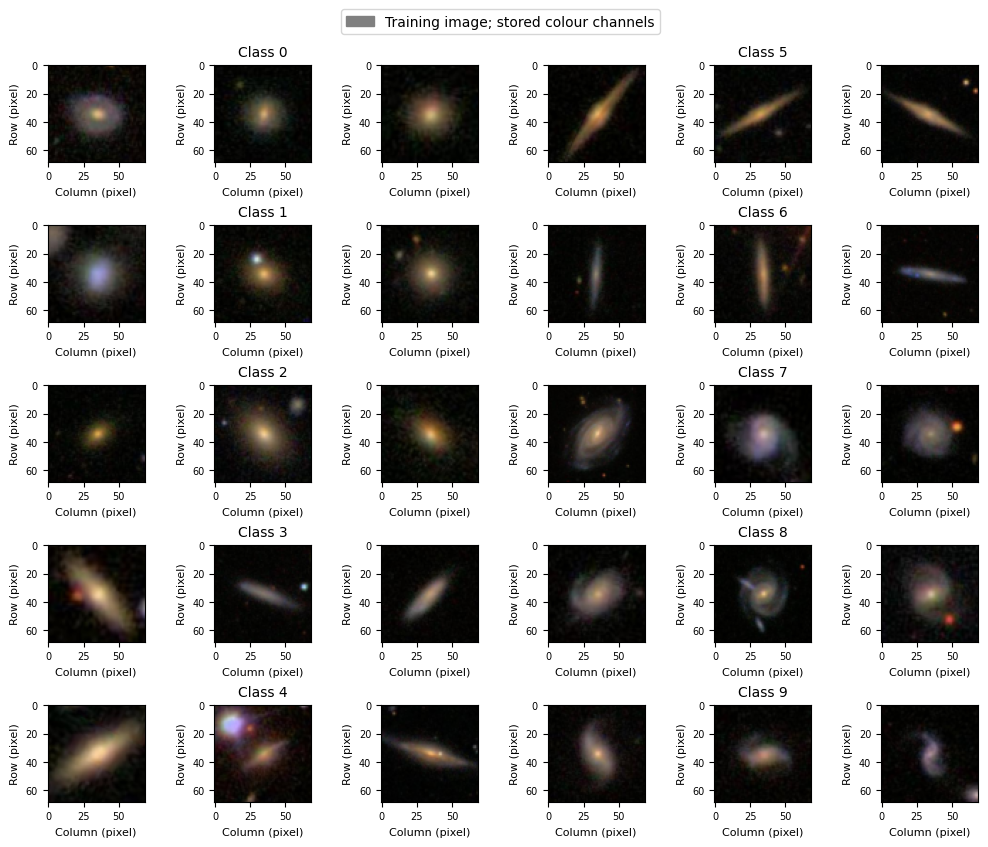
\includegraphics[width=0.86\linewidth]{figures/classes.png}
\caption{Three training images per class.}
\end{figure}

\Needspace{4\baselineskip}

\subsection*{2.2(a). Sky noise}

For each training image and band, I used the outer four-pixel frame (1,040 pixels) to find the median sky, standard deviation, and

\[
\sigma_{\rm MAD}=1.4826\,\operatorname{median}(|I-\operatorname{median}(I)|).
\]

{\small\setlength{\tabcolsep}{4pt}
\begin{tabularx}{\linewidth}{|L|L|L|L|}
\hline
\rowcolor{black!8}
\textbf{Band} & \textbf{Median sky} & \textbf{Median standard deviation} & \textbf{Median MAD noise} \\ \hline
g & 6 & 5.99 & 4.45 \\ \hline
r & 6 & 5.21 & 2.97 \\ \hline
i & 3 & 4.51 & 2.97 \\ \hline
\end{tabularx}\par}

Neighbors and galaxy outskirts raise the standard deviation more than the MAD. The middle-band sky's 5th--95th percentile range is 3--12, so one sky value wouldn't suit every image.

\begin{figure}[H]
\centering
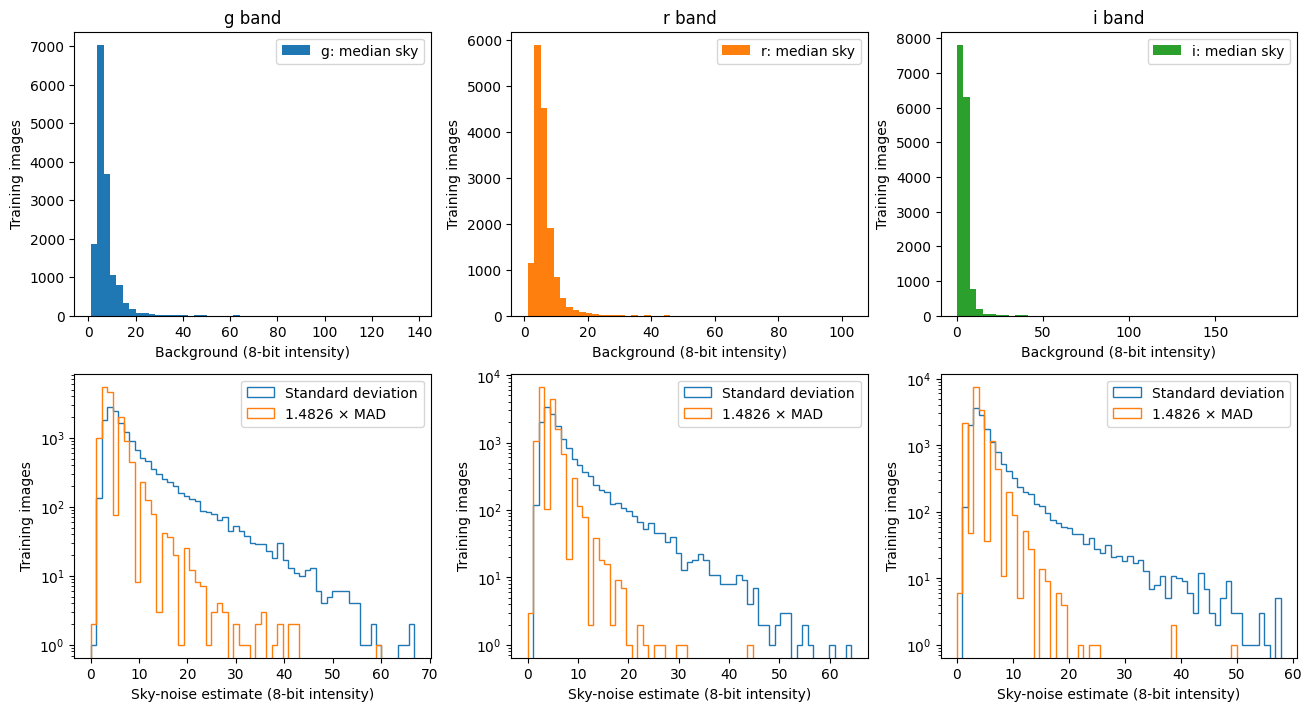
\includegraphics[width=0.91\linewidth]{figures/sky-noise.png}
\caption{Sky levels above, and noise estimates below.}
\end{figure}

\Needspace{4\baselineskip}

\subsection*{2.2(b). Signal-to-noise ratio}

I used the middle band and a radius-8 aperture centered at $(34,34)$, containing 197 pixels:

\[
\mathrm{S/N}=\frac{\sum_{p\in A}(I_{p,r}-b_r)}{\sigma_{{\rm sky},r}\sqrt{197}}.
\]

Some MADs are zero, so I set a minimum noise of $1/\sqrt{12}$, the one-count rounding noise. Class 6 has the lowest median S/N (\textbf{363.5}) and flux (\textbf{12,348}); class 7 has the highest median S/N (\textbf{532.0}). Class 6 looks fainter here, though distance and size also matter. This estimate omits shot noise and pixel correlations.

\begin{figure}[H]
\centering
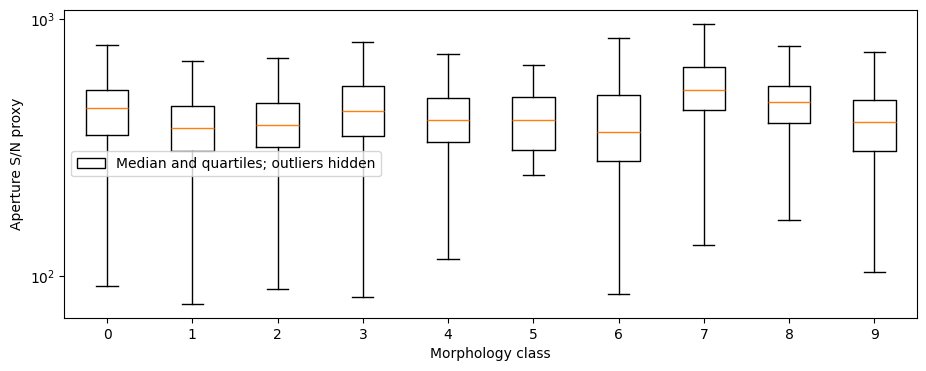
\includegraphics[width=0.85\linewidth]{figures/signal-to-noise.png}
\caption{S/N medians and quartiles by class; outliers are hidden.}
\end{figure}

\Needspace{4\baselineskip}

\subsection*{2.2(c). Contamination and clipping}

I flagged three or more touching border pixels above $b_r+5\max(\sigma_{{\rm MAD},r},1)$, including diagonals. \textbf{61.70\%} of images pass; outskirts and noise can also trigger this. \textbf{0.001758\%} of spatial pixels have a channel at 255. Neighbors bias the sky, while clipping and rounding erase brightness differences. Clipping in these files doesn't necessarily mean detector saturation.

\begin{figure}[H]
\centering
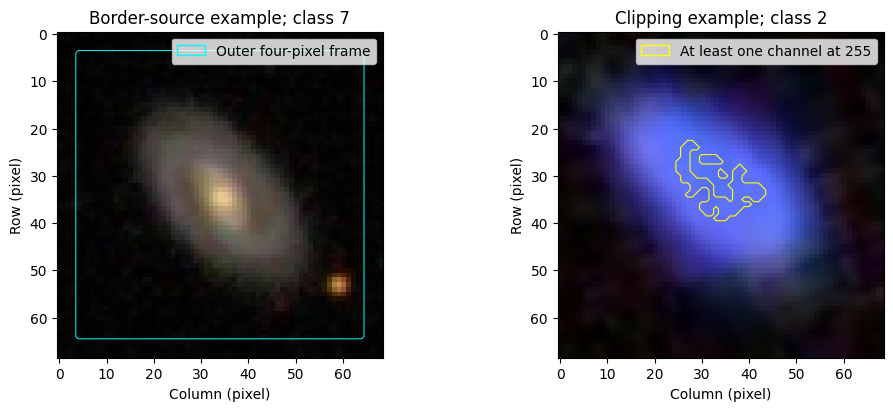
\includegraphics[width=0.76\linewidth]{figures/contamination.png}
\caption{A flagged border source and an example of clipping.}
\end{figure}

\Needspace{4\baselineskip}

\subsection*{2.2(d). Label noise}

I expect confusion between 1/2, 2/3, 4/5/6, and 7/8/9, plus class 0 and smooth galaxies when arms are faint. Volunteers can disagree, so even a sensible prediction can fail against the test label. We would need vote information to estimate an accuracy ceiling.

Cropping, sky subtraction, and averaging can help with unwanted light and noise. They can't restore clipped detail or fix uncertain labels.

\Needspace{4\baselineskip}

\subsection*{2.3(a). Crop}

The average sky-subtracted training image has most of its light near the center. Using one-pixel radial bins, the \textbf{48 by 48} crop (\texttt{10:58}) keeps \textbf{91.15\%, 91.29\%, 90.62\%} of positive stacked light in g/r/i. I accepted losing some outskirts to remove border sky and contamination. Large or off-center galaxies can lose more.

\Needspace{4\baselineskip}

\subsection*{2.3(b). Normalization}

After converting to float32 and subtracting the sky, I used

\[
z_{p,c}=\frac{I_{p,c}-b_c-\mu_c}{s_c}.
\]

Training means are \textbf{(38.8693, 32.6744, 26.2158)} and standard deviations \textbf{(44.5335, 37.3249, 31.6007)}. After preprocessing, means are within $2\times10^{-8}$ of zero and standard deviations are \textbf{1.0000}. I reuse the training values for validation and test to avoid data leakage.

Dividing by each image's brightest pixel removes overall brightness and is sensitive to neighbors. Doing it separately per band also removes color. I kept a shared scale because brightness tells us how visible the galaxy is.

\Needspace{4\baselineskip}

\subsection*{2.3(c). Background subtraction}

I subtracted each band's frame median because sky levels vary. Bright pixels affect it less than the mean, though a large galaxy can still bias it high. I used no smoothing or sharpening. The processed examples use a color scale for the middle band because values can be negative.

\begin{figure}[H]
\begin{minipage}[t]{0.4\linewidth}
\centering\vspace{0pt}
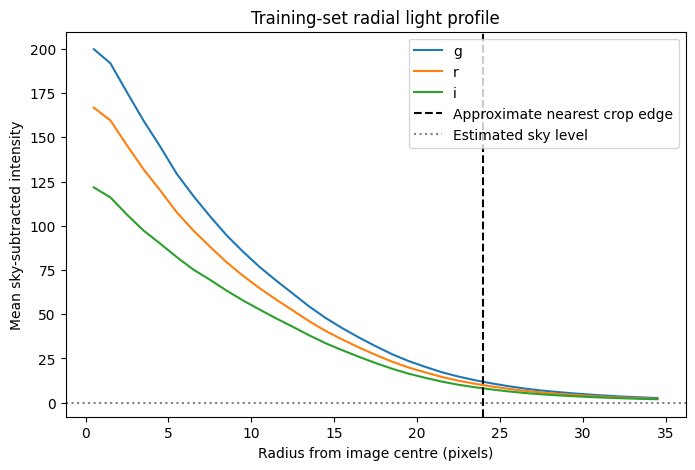
\includegraphics[width=\linewidth]{figures/radial-profile.png}
\caption{Average radial profile; the dashed line marks the crop edge.}
\end{minipage}
\hfill
\begin{minipage}[t]{0.58\linewidth}
\centering\vspace{0pt}
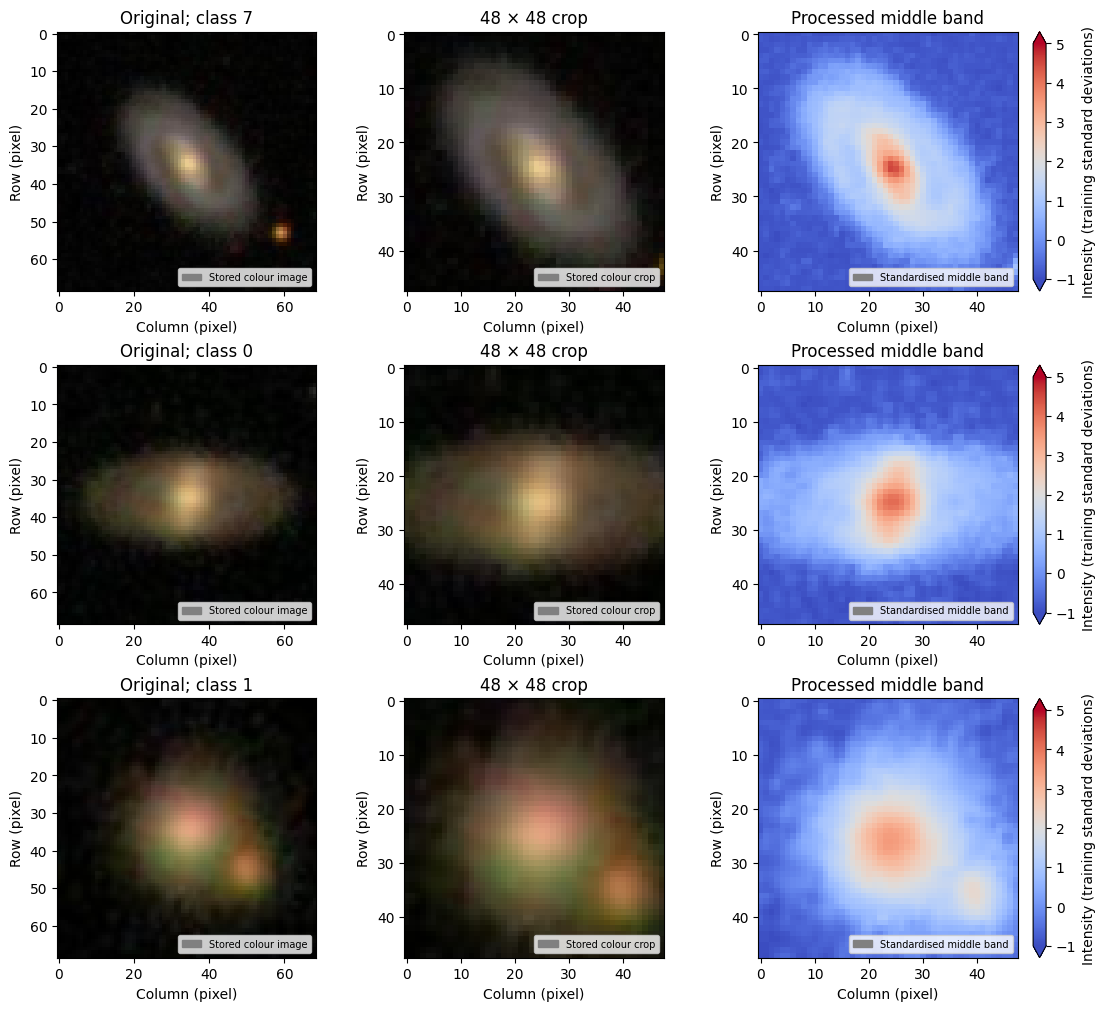
\includegraphics[width=\linewidth]{figures/preprocessing.png}
\caption{Original images, crops, and normalized middle bands.}
\end{minipage}
\end{figure}

\Needspace{4\baselineskip}

\subsection*{2.3(d). Class imbalance}

I used class-weighted cross-entropy, $w_c=N_{\rm train}/(10n_c)$, and shuffled batches. Plain accuracy favors common classes, so I also report \textbf{balanced accuracy}, the average class recall. Weighting gives rare classes more say, but class 5 still has only two test examples.

\Needspace{4\baselineskip}

\subsection*{2.4. Augmentation}

{\normalsize\setlength{\tabcolsep}{4pt}
\begin{tabularx}{\linewidth}{|p{0.22\linewidth}|p{0.17\linewidth}|L|}
\hline
\rowcolor{black!8}
\textbf{Transformation} & \textbf{Use it?} & \textbf{Reason} \\ \hline
Arbitrary rotation & Carefully & Same label, but interpolation/cropping can lose detail. \\ \hline
$90^\circ$ rotations & Yes & Same label, no interpolation. \\ \hline
Horizontal/vertical flips & Yes & Labels don't distinguish spiral handedness. \\ \hline
Small shifts & Yes & Position isn't morphology, unless the crop cuts it off. \\ \hline
Zoom & Small amounts & Changes apparent size and visible detail. \\ \hline
Relative band intensity & No random changes & Color reflects stars, dust, and redshift. \\ \hline
Blur & For known seeing & Can erase arms and bulges. \\ \hline
\end{tabularx}\par}

I would start with flips and right-angle rotations. The required baseline uses \textbf{no augmentation}.

\Needspace{5\baselineskip}

\section*{Part 3 - FCNN and CNN comparison}



\Needspace{4\baselineskip}

\subsection*{Training settings}

All models use the same data, preprocessing, weighted loss, Adam (\textbf{0.001}), batch size \textbf{128}, and at most \textbf{50 epochs}. Early stopping waits \textbf{5} epochs without lower validation loss, then restores the best weights. Baseline seeds are \textbf{11, 22, 33}; scrambled runs use \textbf{11}. No augmentation or added weight decay.

I timed training and validation on an \textbf{Intel Core i7-13700H CPU}, using four threads and PyTorch 2.14.1+cpu. Preprocessing and saving are excluded. The code synchronizes CUDA if a GPU is used.

\Needspace{4\baselineskip}

\subsection*{3.1. Baseline results}

The target is FCNN-matched's best validation accuracy, \textbf{61.41\%}. The main scores and times are in Part 4(a).

{\small\setlength{\tabcolsep}{4pt}
\begin{tabularx}{\linewidth}{|L|L|L|L|}
\hline
\rowcolor{black!8}
\textbf{Model} & \textbf{Target reached} & \textbf{Epochs to target} & \textbf{Selected epoch} \\ \hline
FCNN-matched & 1/3 & 13.00 (one run) & 8.67 \(\pm\) 1.53 \\ \hline
FCNN-large & 2/3 & 6.50 \(\pm\) 2.12 & 3.33 \(\pm\) 0.58 \\ \hline
CNN & 3/3 & 12.67 \(\pm\) 2.52 & 12.33 \(\pm\) 0.58 \\ \hline
\end{tabularx}\par}

Values are mean \(\pm\) sample standard deviation. Target times and epochs count only successful runs and use the first crossing. One successful run has no across-seed deviation. Selected epochs have the lowest validation loss. The code's parameter counts agree with T1.

\Needspace{4\baselineskip}

\subsection*{3.1. Loss curves}

For CNN seed 11, training loss falls \textbf{1.024\(\to\)0.820} over epochs 12--17 while validation loss rises \textbf{1.342\(\to\)1.468}: it overfits too. I kept epoch 12. Each of the three class-5 validation images has weight about \textbf{127}, making validation noisy. Dropout is on only during training.

\begin{figure}[H]
\centering
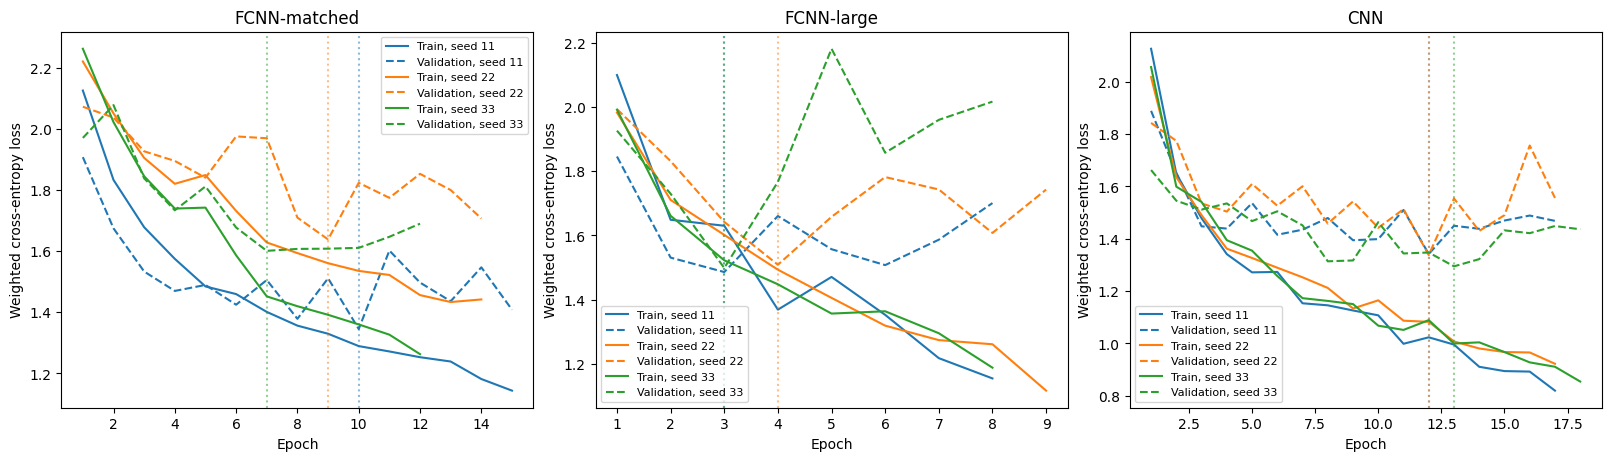
\includegraphics[width=1\linewidth]{figures/loss-curves.png}
\caption{Training and validation loss. Dotted lines mark the restored epochs.}
\end{figure}

\Needspace{4\baselineskip}

\subsection*{3.1. Confusion matrices}

The best seeds by validation loss are \textbf{11, 11, 33} for matched, large, and CNN. Their most common mistake is \textbf{class 2 as class 1}: \textbf{297, 331, 113} images. The CNN swaps 41 tight and 35 medium spirals into each other's classes. These match the expected overlaps. It also misses both class-5 images and gets only \textbf{20.6\%} of class 0 right.

\begin{figure}[H]
\centering
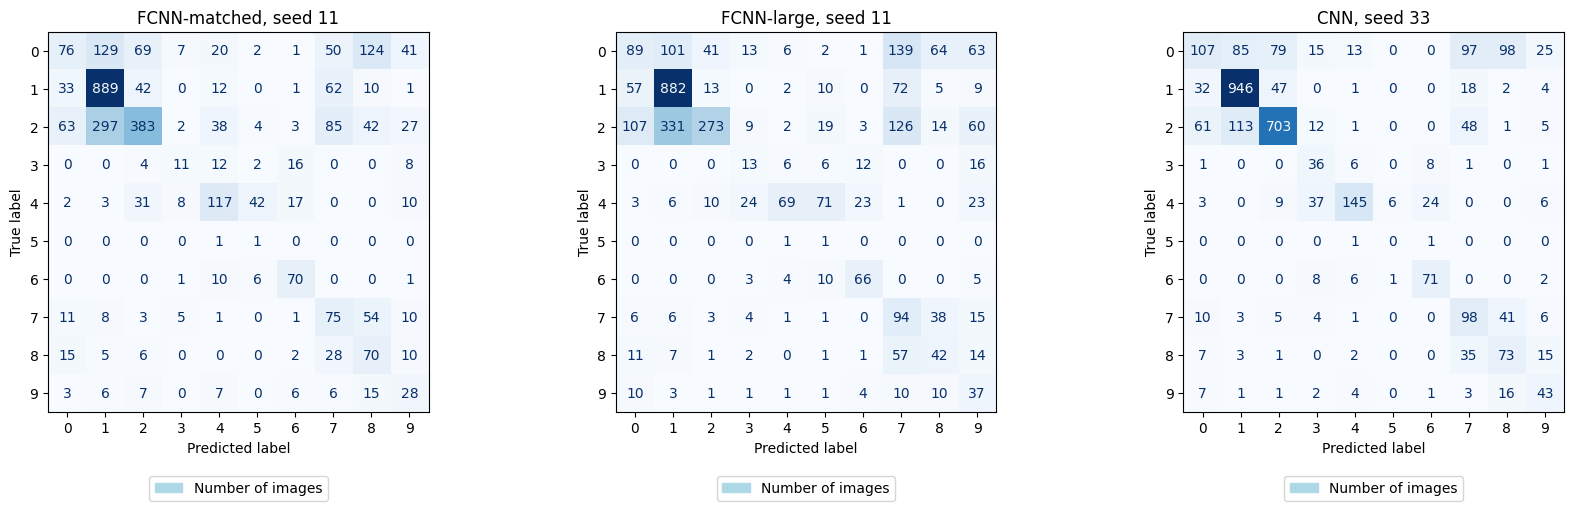
\includegraphics[width=1\linewidth]{figures/confusion-matrices.png}
\caption{Best seed of each model. Rows are true classes; columns are predictions.}
\end{figure}

\Needspace{4\baselineskip}

\subsection*{3.1. ROC curves}

Using softmax scores, class-2/class-7 AUCs are \textbf{0.780/0.889} (matched), \textbf{0.778/0.877} (large), and \textbf{0.912/0.929} (CNN). The CNN ranks these classes best; AUC isn't the same as ten-class accuracy.

\begin{figure}[H]
\centering
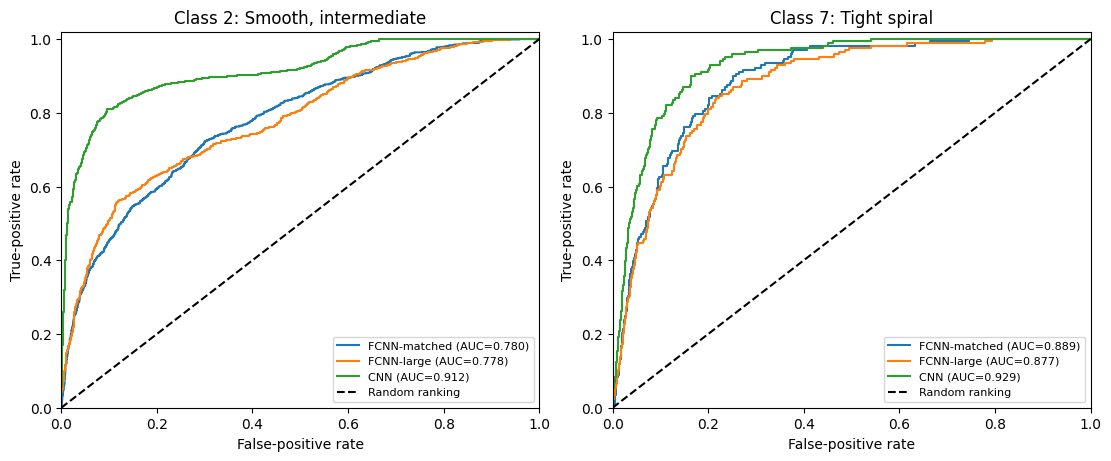
\includegraphics[width=0.9\linewidth]{figures/roc-curves.png}
\caption{ROC curves for classes 2 and 7.}
\end{figure}

\Needspace{4\baselineskip}

\subsection*{3.2. Shifted images}

I shifted each crop by $d=0,2,4,6,8$ in a random direction (seed \textbf{3200}), rounded to pixels. All models use the same shifts, original sky estimates, normalization, and weights.

{\normalsize\setlength{\tabcolsep}{4pt}
\begin{tabularx}{\linewidth}{|L|L|L|}
\hline
\rowcolor{black!8}
\textbf{Model} & \textbf{Accuracy at $d=8$ (\%)} & \textbf{Drop from $d=0$ (points)} \\ \hline
FCNN-matched & 20.25 \(\pm\) 3.64 & 30.28 \\ \hline
FCNN-large & 17.25 \(\pm\) 3.74 & 34.70 \\ \hline
CNN & 30.79 \(\pm\) 4.85 & 27.15 \\ \hline
\end{tabularx}\par}

The CNN loses less, as predicted, but isn't invariant. Pooling boundaries, position-specific dense weights, and cut-off light still matter. Rounding slightly changes the distances from $d$.

\Needspace{4\baselineskip}

\subsection*{3.3. Scrambled-image results}

One shuffle (seed \textbf{2026}) is shared by training, validation, and test, keeping each pixel's color channels together. Both models are retrained with seed \textbf{11} and compared with their seed-11 baselines.

{\small\setlength{\tabcolsep}{4pt}
\begin{tabularx}{\linewidth}{|L|L|L|L|}
\hline
\rowcolor{black!8}
\textbf{Model} & \textbf{Original accuracy (\%)} & \textbf{Scrambled accuracy (\%)} & \textbf{Change (points)} \\ \hline
FCNN-matched & 52.63 & 50.40 & -2.23 \\ \hline
CNN & 55.05 & 63.68 & +8.63 \\ \hline
\end{tabularx}\par}

The FCNN barely changes, as expected. \textbf{The CNN improves, so my prediction was wrong.} Its dense layer can still combine shuffled information. One run doesn't show that scrambling helps: baseline CNN scores vary by about nine points, and rare validation images affect early stopping. I would need more seeds and shuffles to check.

\begin{figure}[H]
\begin{minipage}[t]{0.48\linewidth}
\centering\vspace{0pt}
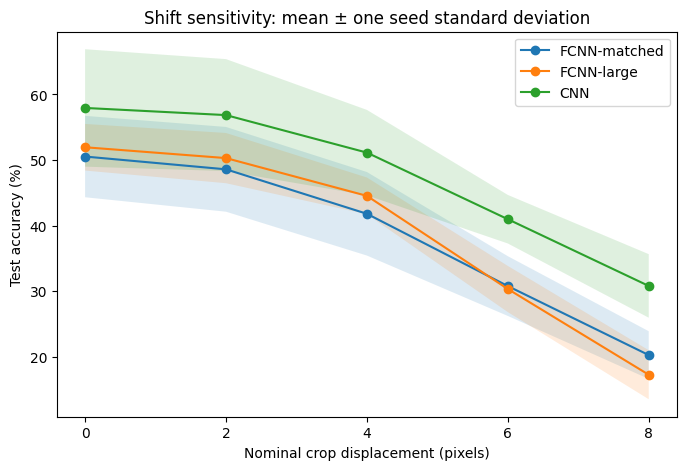
\includegraphics[width=\linewidth]{figures/shifted-images.png}
\caption{Shift accuracy: mean and standard deviation across seeds.}
\end{minipage}
\hfill
\begin{minipage}[t]{0.48\linewidth}
\centering\vspace{0pt}
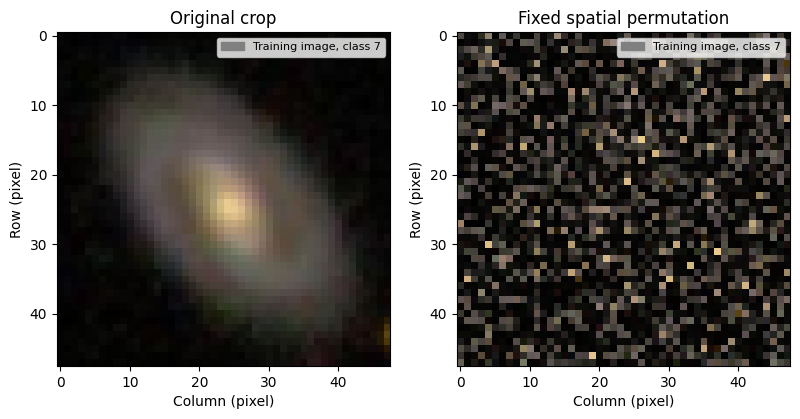
\includegraphics[width=\linewidth]{figures/scrambled-image.png}
\caption{One image before and after shuffling.}
\end{minipage}
\end{figure}

\begin{minipage}{\linewidth}
\raggedright
\setlength{\parskip}{5pt}
\setlength{\extrarowheight}{1pt}

\Needspace{5\baselineskip}

\section*{Part 4 - Discussion}

\label{discussion-start}



\Needspace{4\baselineskip}

\subsection*{4(a). Performance and speed}

I would pick the CNN for accuracy, but it takes much longer on this CPU. It reaches the target in all three runs, versus one and two for the FCNNs. It isn't faster in wall-clock time.

{\fontsize{9}{11}\selectfont\setlength{\tabcolsep}{4pt}
\begin{tabularx}{\linewidth}{|L|C|C|C|C|C|C|}
\hline
\rowcolor{black!8}
\textbf{Model} & \textbf{Accuracy (\%)} & \textbf{Balanced accuracy (\%)} & \textbf{Parameters} & \textbf{MACs / image} & \textbf{Seconds / epoch} & \textbf{Seconds to target} \\ \hline
\shortstack[l]{FCNN-\\matched} & \shortstack{50.53\\$\pm 6.21$} & \shortstack{44.73\\$\pm 2.26$} & 168,162 & 168,064 & \shortstack{1.61\\$\pm 0.49$} & 27.96 \\ \hline
\shortstack[l]{FCNN-\\large} & \shortstack{51.95\\$\pm 3.56$} & \shortstack{44.72\\$\pm 0.54$} & 1,803,914 & 1,803,520 & \shortstack{2.59\\$\pm 0.36$} & \shortstack{15.56\\$\pm 5.14$} \\ \hline
CNN & \shortstack{57.95\\$\pm 8.96$} & \shortstack{52.04\\$\pm 4.26$} & 171,754 & 6,451,840 & \shortstack{36.26\\$\pm 0.67$} & \shortstack{466.31\\$\pm 100.69$} \\ \hline
\end{tabularx}\par}

Mean \(\pm\) sample standard deviation; parameters and MACs are fixed. Target times include only successful runs (one for FCNN-matched).



\Needspace{4\baselineskip}

\subsection*{4(b). What about these images helps?}

The CNN handled shifts better. The crop kept \textbf{91\%} of the average image's light, so most structure is near the center. Small filters can find parts of arms and bulges for later layers to combine, though scrambling didn't show this benefit. Noise (\textbf{2.97--5.99 counts}) and contamination justify preprocessing; I didn't separately test pooling.

\Needspace{4\baselineskip}

\subsection*{4(c). Five magnitudes}

I would use a small FCNN for $(u,g,r,i,z)$: there is no 2D image structure. A 1D CNN assumes patterns can move between bands without changing meaning, which doesn't fit five fixed, unevenly spaced filters. It makes more sense for a densely sampled spectrum.

\Needspace{4\baselineskip}

\subsection*{4(d). What I would change first}

I would check labels and get more rare-class examples first. The CNN misses both class-5 images and gets only \textbf{20.6\%} of class 0 right, despite its reasonable S/N. Noise, clipping, resolution, and other sources limit what is visible. A bigger network can't recover missing detail or settle unclear labels.

\label{discussion-end}

\Needspace{5\baselineskip}

\subsection*{AI Usage}

I used OpenAI Codex for help with the theory, code, debugging, and writing. The numbers come from running the notebook.

\end{minipage}
\end{document}
